\subsection{Client-Server}
Die \first{Pipes} des \name{pipes and filters} Pattern werden zu einem
\first{Server} zusammengefasst und bilden das statische Ausführungsgerüst.
Ein \first{Client} stellt einen \first{Filter} des \name{pipes and filters}
Pattern dar.
Die einzelnen Clients sind dynamisch und somit nicht Teil der
statischen Kernanwenung.
\index{Filter}
\index{Step}
\index{Client}
Es können beliebig viele Clients am Server anmeldet werden, wodurch die
eigentliche Pipeline aufgebaut wird.
\todo{ein alles in allem doofer Absatz\ldots}

\paragraph{Server}
Die Anforderungen an den Server gliedern sich in zwei Teilbereiche:
\begin{description}
\item[Organisation und Synchronisation der Client Ausführung]
Die Ausfürhrung der angemeldeten Steps kann sequenziell oder
parallel erfolgen, je nachdem, welche \first{execution preconditions} für den
jeweiligen Step erforderlich sind und ob die zur Ausführung benötigten Daten
eventuell erst durch einen anderen Step bereitgestellt werden müssen.
Vor der eigentlichen Ausführung wird der Server somit zum einen die
\name{execution preconditions} prüfen, zum anderen, ob der Step überhaupt zur Ausführung
gebracht werden muss, oder ob die zu erwartenden Ergebnisse bereits in selber
oder in anderer Form vorhanden sind.
\item[Datenverwaltung] Die Ergebnisse der einzelnen Steps werden zentral durch
den Server verwaltet.
Zum einen synchronisiert der Server die Zugriffe auf die Daten, zum anderen
werden diese persistiert, um bei einer gewollten oder ungewollten Unterbrechung
der Pipeline Datenverlust zu verhindern.
\end{description}

\paragraph{Client}
Auf der Clientseite stehen die einzelnen \first{Filter} der Pipeline, im
folgenden \first{Steps} genannt \todo{hmmm}. Jeder Step soll technisch
gesehen einem oder mehreren OSGi-Bundles entsprechen.
\index{Step}
\index{Filter}
\index{Client}
\index{Bundle}
\index{OSGi-Bundle}
Wird das Bundle durch das OSGi-Framework gestartet, soll sich der Step am Server
anmelden. Der Step stellt dabei entsprechende \name{call-back-Methoden} für die
eigentliche Ausführung, Überprüfung der \name{execution preconditions} und
Ähnlichem bereit.
\index{Server}
\index{OSGi Framework}
\index{call back method}
Wann diese Methoden aufgerufen werden, obliegt so allein
dem Server.
Als Prameter der call back methoden wird die Sequenz, sowie das zentrale
Datenobjekt, im Folgenden \first{Data bean} \todo{hmmm} genannt,
übergeben.

%%
%\begin{figure}[htbp]
%	\begin{center}
%		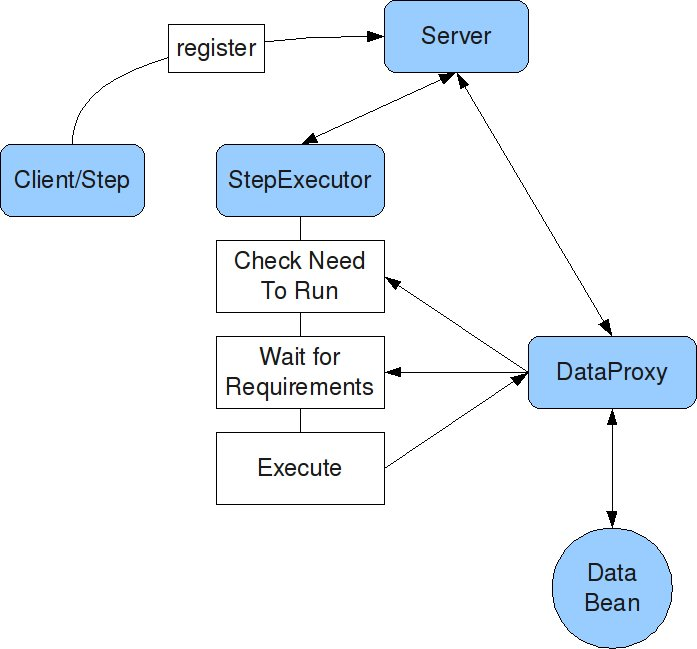
\includegraphics[scale=0.6]{pics/programOrganisationOverview3ScaledWithAlpha.jpg}
%	\caption[Design 1]{
%	\textbf{Design 1.}
%	something. \todo{Teilung von Server hier noch nicht erwähnt. Evtl. Teil der
%	Umstzung}}
%	\end{center}
%	\label{fig:programOrganisationOverview3ScaledWithAlpha}
%\end{figure}